\documentclass[12pt]{article}
\usepackage[margin=2.5cm]{geometry}
\usepackage{enumerate}
\usepackage{amsfonts}
\usepackage{amsmath}
\usepackage{fancyhdr}
\usepackage{amsmath}
\usepackage{amssymb}
\usepackage{amsthm}
\usepackage{mdframed}
\usepackage{graphicx}
\usepackage{subcaption}
\usepackage{listings}
\usepackage{xcolor}
\usepackage{booktabs}
\usepackage[utf]{kotex}

\definecolor{codegreen}{rgb}{0,0.6,0}
\definecolor{codegray}{rgb}{0.5,0.5,0.5}
\definecolor{codepurple}{rgb}{0.58,0,0.82}
\definecolor{backcolour}{rgb}{0.95,0.95,0.92}

\lstdefinestyle{mystyle}{
    backgroundcolor=\color{backcolour},
    commentstyle=\color{codegreen},
    keywordstyle=\color{magenta},
    numberstyle=\tiny\color{codegray},
    stringstyle=\color{codepurple},
    basicstyle=\ttfamily\footnotesize,
    breakatwhitespace=false,
    breaklines=true,
    captionpos=b,
    keepspaces=true,
    numbers=left,
    numbersep=5pt,
    showspaces=false,
    showstringspaces=false,
    showtabs=false,
    tabsize=1
}

\lstset{style=mystyle}

\begin{document}
\title{CSC148 Worksheet 9 Solution}
\author{Hyungmo Gu}
\maketitle

\section*{Question 1}
\begin{figure}[h!]
    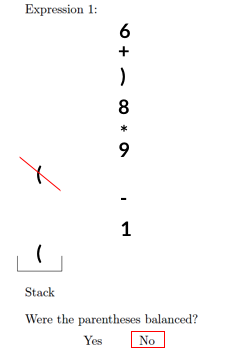
\includegraphics[width=0.45\textwidth]{images/worksheet_9_q1a_solution.png}\hfill
    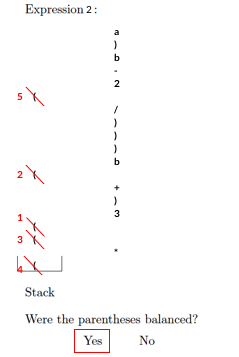
\includegraphics[width=0.45\textwidth]{images/worksheet_9_q1b_solution.png}\hfill
\end{figure}

\begin{figure}[h!]
    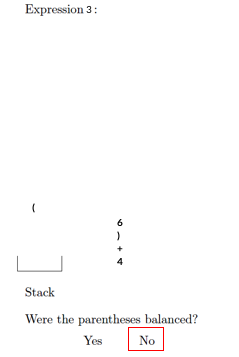
\includegraphics[width=0.45\textwidth]{images/worksheet_9_q1c_solution.png}\hfill
\end{figure}

\newpage

\section*{Question 2}
\begin{enumerate}[a.]
    \item

    For each character being received,

    \begin{enumerate}[1.]
        \item If the character is left parenthesis, then we need to store it in stack using \textit{push()} method
        \item If the character is right parenthesis
        \begin{enumerate}[1.]
            \item First, check for the non-emptiness of stack.
            \item If the list is not empty, then we need to pop an element form stack.
            \item If list is empty, then we need to raise error.
        \end{enumerate}
        \item If the character is other than left or right parenthesis, then pass the character.
    \end{enumerate}
\end{enumerate}

\section*{Question 3}

\section*{Question 4}

\end{document}